\documentclass[TheoreticalPhy_ModB.tex]{subfiles}
\begin{document}

\chapter{Non abelian Gauge Theories}
\textsf{Maggiore sec. 10.1; Peskin sec. 15.1; Schwartz sec. 25.Intro; Mandl sec. 11.Intro, 11.1}\\

In this chapter we introduce non-abelian gauge theories, or Yang-Mills theories. Their importance stems from the fact that strong interactions are described by a non-abelian gauge theory with gauge group $SU(3)$, known as quantum chromodynamics or QCD, while the electromagnetic and weak interactions are unified in a gauge theory with gauge group $SU(2)\times U(1)$, the electroweak theory. Together, QCD and the electroweak theory form the Standard Model, which to date reproduces all known experimental results of particle physics, up to energies of the order of a few hundred GeV.

A full presentation of the Standard Model is beyond the scope of this course. In this and the next chapter we will however introduce two of its main ingredients, namely Yang-Mills theories and the Higgs mechanism. 

Non-abelian gauge theories\footnote{For a description of Gauge groups, Lie Algebras and their representation, see \textsf{Peskin sec. 15.4; Schwartz sec. 25.1}}, beside having an extraordinary experimental success, have also a very rich theoretical structure, at the classical and especially at the quantum level. Within the scope of this course, we can only limit ourself to just a few elementary aspects, in particular, we will discuss how to generalize gauge transformations to non-abelian groups and how to write the corresponding invariant Lagrangians. 

As a first step, it is useful to rewrite the abelian gauge transformation of electrodynamics in a form more suitable for generalization. 
We already know that the Lagrangian of QED is invariant under a very large group of transformations, allowing an independent symmetry transformation at every point in spacetime. This invariance is the famous \emph{gauge symmetry} of QED. From the modern viewpoint, however, gauge symmetry is not an incidental curiosity, but rather the fundamental principle that determines the form of the Lagrangian. Let us now review the elements of the theory, taking a modern viewpoint. 

We begin with the complex-valued Dirac field $\psi(x)$, and stipulate that our theory should be invariant under the transformation
\[\psi(x)\quad\to\quad e^{iq\alpha(x)}\psi(x)=\Omega(x)\psi(x)\]
where $\Omega(x)=e^{iq\alpha(x)}$ is the representation of the $U(1)$ transformation. The transformation of the gauge field instead is 
\[A_\mu(x)\quad\to\quad A_\mu(x)-\partial_\mu\alpha(x)=\Omega(x)A_\mu(x)\Omega^\dagger(x)-\frac iq(\partial_\mu\Omega)\Omega^\dagger\]
where in the last step we used the propriety $\Omega^{-1}(x)=\Omega^\dagger(x)$ that holds since we arae considering the unitary group $U(1)$. 
The coupling between $A_\mu$ and $\psi$ is obtained using the \emph{covariant derivative}, which in the representation to which $\psi$ belongs takes the form
\[D_\mu=(\partial_\mu+iqA_\mu)\]
The important propriety of the covariant derivative is that, even under $x$-dependent transformations, it transforms in the same way as $\psi$:
\[D_\mu\psi\quad\to\quad \Omega(D_\mu\psi)\]
Using covariant derivatives there is a very simple way to construct a theory with local $U(1)$ invariance: we start from a theory with global $U(1)$ invariance and we just replace all the ordinary derivatives with covariant derivatives. This method of coupling matter to the electromagnetic field is know as \emph{minimal coupling}. Non-minimal coupling are also possible, but they are characterized by coupling constant with dimensions of the inverse powers of mass. If we consider the example of the Fermi theory, we understand that couplings with inverse mass dimensions are less fundamental than dimensionless couplings, and emerge as the low-energy limit of some more fundamental dimensionless coupling. Therefore, it is the minimal coupling that we want to generalize. \\
Notice that, since covariant derivative $D_\mu\psi$ has same proprieties of the field $\psi$, we have
\[D_\mu D_\nu\psi\quad\to\quad \Omega(D_\mu D_\nu\psi)\]
However, the commutator between covariant derivatives is not a derivative at all, since in general (for any gauge theory) it acts multiplicatively on the field $\psi$:
\begin{equation}\label{eqn:prop-F-covdev-rel}
-\frac iq[D_\mu,D_\nu]\psi=F_{\mu\nu}\psi
\end{equation}
where we introduced the structure $F_{\mu\nu}=\partial_\mu A_\nu-\partial_\nu A_\mu$. Let's consider the transformation propriety of this structure:
\[F_{\mu\nu}\psi\quad\to\quad -\frac iq\Omega[D_\mu,D_\nu]\psi=\Omega F_{\mu\nu}\psi\]
this means that 
\begin{equation}\label{eqn:F-tensor-transform}
F_{\mu\nu}\quad\to\quad\Omega F_{\mu\nu}\Omega^\dagger
\end{equation}
and therefore this structure is a tensor. 

If the simple geometrical construction we have just presented yield Maxwell's theory of electrodynamics, then surely it must be possible to construct other interesting theories by starting from more general geometrical principles. We want to generalize the above transformations to the case where $\Omega$ belong to a non-abelian group $G$, rather then just to $U(1)$, and we want to construct a Lagrangian invariant under such local transformations. We will limit ourselves to the case $G=SU(N)$, although the construction is very general; $G$ is called the \textbf{gauge group}.

We start considering a fermion field\footnote{For definiteness we take $\psi_i$ to be Dirac fermions, but all the subsequent considerations are very general and apply to any matter fields, e.g. to bosonic fields or to Weyl fermions.} in $N$-dimensional fundamental representation\footnote{Notice that this construction is similar to the one we used for flavours. Nevertheless, this time we require a local symmetry, not only global.}
\[\Psi=\begin{pmatrix}\psi_1\\\vdots\\\psi_N\end{pmatrix}\]
The fact that $\Psi$ transform in the $N$-dimensional fundamental representation means that, under a gauge transformation
\[\Psi(x)\quad\to\quad\Psi'(x)=\Omega(x)\Psi(x)\]
The transformation matrix $\Omega\in SU(N)$ can be written as
\[\Omega(x)=\exp{ig\hat\alpha(x)}\]
where $\hat\alpha$ is a function that can be written in terms of the $N^2-1$ generators $T^a$ of the group $SU(N)$
\begin{equation}\label{eqn:alpha-deco-gauge}
\hat\alpha(x)=\alpha^a(x)T^a
\end{equation}
To construct an invariant Lagrangian, we introduce a set of gauge fields $A_\mu^a$ labeled by an index $a$, with one gauge field for each generator of the gauge group; the $A_\mu^a$ are called \textbf{non-abelian gauge fields}.   In particular, $SU(N)$ has $N^2-1$ generators, so we have three gauge fields for $SU(2)$ and eight gauge fields for $SU(3)$. We introduce the matrix field
\begin{equation}\label{eqn:matrix-vector-pot-gauge}
\hat A_\mu(x)=\sum_{a=1}^{N^2-1}A_\mu^a(x)T^a
\end{equation}
The summation over $a$ will be omitted from now on, it should be introduced each time there are two indeces $a$ in the same term. 

We now introduce the covariant derivative on the field $\psi$. The most general form is
\begin{equation}\label{eqn:gauge-cov-deriv}
\hat D_\mu\Psi=(\id_N\partial_\mu+igA_\mu^a(x)T^a)\Psi=(\hat \partial_\mu+ig\hat A_\mu(x))\Psi
\end{equation}
Fields $A_\mu^a$ do not depend on the specific representation we choose\footnote{Just as in electromagnetism the gauge field, and therefore its transformation proprieties, does not know anything about about the representation of the matter field we consider.} for the field $\Psi$ and neither do the covariant derivative $\hat D_\mu$. Even if we use non-fundamental representation $\Psi_R$ of the field (and therefore different generators $T^a_R$) equation eq.~\eqref{eqn:gauge-cov-deriv} does not change. 

\section{The Yang-Mills Lagrangian}

\textsf{Maggiore sec. 10.2; (Peskin sec. 15.2)}\\

The free Dirac Lagrangian 
\[\mathcal L_{\text{free}}=\bar\Psi(i\hat{\slashed\partial}-m)\Psi\equiv\sum_{\alpha=1}^N\bar\psi^\alpha(i(\hat{\slashed\partial}\psi)^\alpha-m\psi^\alpha)\]
is invariant under global $SU(N)$ transformations, since if $\Psi\to\Omega\Psi$ then $\bar\Psi\to\Psi\Omega^\dagger$ and, if $\Omega$ is independent of $x$, it goes through $\partial_\mu$ and cancels against $\Omega^\dagger$. However, if $\Omega$ depends on $x$, performing the transformation we also get a term proportional to $\partial_\mu\Omega$ and this Lagrangian is no longer invariant. 

To construct an invariant Lagrangian, we have to use the covariant derivative, just replacing $\partial_\mu\to D_\mu$ in the free theory, that is 
\begin{equation}\label{eqn:Dirac-lag-gauge}\boxed{
\mathcal L_D=\bar\Psi(i\hat{\slashed D}-m)\Psi\equiv\sum_{\alpha=1}^N\bar\psi^\alpha(i(\hat{\slashed D}\psi)^\alpha-m\psi^\alpha)
}\end{equation}
We can obtain the gauge transformation of $A_\mu$ just requiring the invariance of the Dirac Lagrangian. We impose that 
\[\hat D_\mu\Psi\quad\to\quad\Omega(\hat D_\mu\Psi)\]
We have
\begin{align*}
(\hat D_\mu\Psi)'&=(\hat \partial_\mu+ig\hat A'_\mu(x))\Omega\Psi=((\hat \partial_\mu\Omega)+\Omega\hat \partial_\mu+ig\hat A'_\mu(x))\Psi\\
&\overset{!}{=}\Omega(\hat D_\mu\Psi)=\Omega(\hat \partial_\mu+ig\hat A_\mu(x))\Psi
\end{align*}
and therefore the requirement implies the following gauge transformation for the field $\hat A_\mu$:
\begin{equation}\label{eqn:trn-A-gauge}\boxed{
\hat A_\mu\quad\to\quad\Omega\hat A_\mu\Omega^\dagger+\frac1g(\hat \partial_\mu\Omega)\Omega^\dagger
}\end{equation}
The Lagrangian eq.~\eqref{eqn:Dirac-lag-gauge} contains the fermionic field and its interaction with the gauge fields. The interaction term, which is hidden in the covariant derivative, is
\[\mathcal L_{\text{int}}=g\bar\psi^\alpha \slashed A_\mu^a(T^a)_{\alpha\beta}\psi^\beta\]
and we see that $g$ is a couling constant. We also need a kinetic term for the gauge fields. One might try to define the field strength tensor of each of the gauge fields $A^a_\mu$ as $F_{\mu\nu}^a=\partial_\mu A^a_\nu-\partial_\nu A^a_\mu$, but it is immediate to verify that this quantity does not satisfy any simple transformation property under gauge transformation under eq.~\eqref{eqn:trn-A-gauge}. Instead, a straightforward computation shows that the quantity
\begin{equation}\label{eqn:dfn-F-gauge}\boxed{
\hat F_{\mu\nu}=\hat \partial_\mu \hat A_\nu-\hat \partial_\nu \hat A_\mu-ig[\hat A_\mu,\hat A_\nu]
}\end{equation}
transforms as
\begin{equation}\label{eqn:F-tensor-matr-transform}
F_{\mu\nu}\quad\to\quad\Omega(x)F_{\mu\nu}\Omega^\dagger(x)
\end{equation}
and satisfy the relation
\[-\frac ig[\hat D_\mu,\hat D_\nu]\Psi=F_{\mu\nu}\Psi\]
which are the trivial generalizations of eq.~\eqref{eqn:F-tensor-transform} and eq.~\eqref{eqn:prop-F-covdev-rel}.
Therefore, using the definition eq.~\eqref{eqn:dfn-F-gauge} the tensor $\hat F_{\mu\nu}$ is the generalization of the field strength tensor $F_{\mu\nu}$ we defined for the Maxwell's field. The object $\hat F_{\mu\nu}$ is called \textbf{non-abelian field strength tensor}. From eq.~\eqref{eqn:dfn-F-gauge} ad eq.~\eqref{eqn:matrix-vector-pot-gauge} we see that we can rewrite $\hat F_{\mu\nu}$ as
\[\hat F_{\mu\nu}= F_{\mu\nu}^a T^a\]
with\footnote{Recall that \emph{structure constant} are defined as $[T^a,T^b]=if^{abc}T^c$.}
\begin{equation}\label{eqn:deco-F-tensor}
F_{\mu\nu}^a=\partial_\mu A_\nu^a-\partial_\nu A_\mu^a+gf^{abc}A_\mu^bA_\nu^c
\end{equation}
Now it is easy to construct a gauge-invariant kinetic term for the gauge field; it is given by
\[\mathcal L_{\text{gauge}}=-\frac12\Tr[F_{\mu\nu}F^{\mu\nu}]=-\frac14F_{\mu\nu}^aF^{\mu\nu}_a\]
where $F_{\mu\nu}$ has be taken in the fundamental representation, and we used the fact that $\Tr(T^aT^b)=\delta^{ab}/2$. Under gauge transformations $\Tr F_{\mu\nu}F^{\mu\nu}\to \Tr (\Omega F_{\mu\nu}F^{\mu\nu}\Omega^\dagger)=\Tr F_{\mu\nu}F^{\mu\nu}$ due to the cyclic property of the trace. 

The complete Lagrangian of the $SU(N)$ Yang-Mills theory with Dirac fermions is therefore 
\begin{equation}\label{eqn:YM-lag}\boxed{
\mathcal L_{YM}=\bar\Psi(i\slashed D-m)\Psi-\frac12\Tr F_{\mu\nu} F^{\mu\nu}
}\end{equation}
This Lagrangian is called \textbf{Yang-Mills Lagrangian}. The kinetic term for the gauge field can be rewritten using the vector potential $\hat A_\mu$ as follows
\begin{subequations}\label{eqn:YM-lag-potentials}\begin{align}
\mathcal L_{\text{gauge}}
&=-\frac12\Tr[(\partial_\mu\hat A_\nu-\partial_\nu\hat A_\mu)^2]\\
&\quad-ig\Tr[(\partial_\mu\hat A_\nu-\partial_\nu\hat A_\mu)[A^\mu,A^\nu]]\label{eqn:YM-lag-potentials-3int}\\
&\quad+\frac{g^2}2\Tr[[\hat A_\mu,\hat A_\nu][\hat A^\mu,\hat A^\nu]]\label{eqn:YM-lag-potentials-4int}
\end{align}\end{subequations}
Observe, from eq.~\eqref{eqn:YM-lag-potentials}, that the term $F^2$ contains not only the standard kinetic term of the gauge fields, but also an interaction vertex with three gauge bosons, proportional to $g$, and a vertex with four gauge bosons, proportional to $g^2$. This interactions represented in following figures:
\[
\begin{tikzpicture}[baseline=(e0)]
	\begin{feynman}[small]
		\vertex(e0);
		\vertex[below left=of e0](e1);
		\vertex[below right=of e0](e2);
		\vertex[above=0.9cm of e0](e3);
		\diagram*{
			(e1)--[boson](e0)--[boson](e2),
			(e0)--[boson](e3),
		};
	\end{feynman}
\end{tikzpicture}
\propto g
\hspace{3cm}
\begin{tikzpicture}[baseline=(e0)]
	\begin{feynman}[small]
		\vertex(e0);
		\vertex[below left=of e0](e1);
		\vertex[below right=of e0](e2);
		\vertex[above left=of e0](e3);
		\vertex[above right=of e0](e4);
		\diagram*{
			(e1)--[boson](e0)--[boson](e2),
			(e3)--[boson](e0)--[boson](e4),
		};
	\end{feynman}
\end{tikzpicture}
\propto g^2
\]
Observe also that gauge invariance has fixed the three-boson, four-boson, and boson-fermion-fermion vertices in terms of a single parameter, the gauge coupling $g$.


\subsubsection{Adjoint representation of the field strength tensor}
\textsf{Maggiore sec. 10.4}\\

Finally, notice that eq.~\eqref{eqn:F-tensor-matr-transform} means that the tensor $\hat F_{\mu\nu}$ transforms with the adjoint representation of the group. Let's take an infinitesimal gauge transformation, i.e. $\Omega(x)\simeq\id+ig\hat \alpha(x)+o(\hat \alpha^2(x))$, then
\begin{equation}\label{eqn:fund-rep-field-analogy}
\Psi\quad\to\quad\Omega\Psi=\p{e^{ig\alpha^aT^a}}\Psi\simeq\Psi+ig\alpha^aT^a\Psi
\end{equation}
Under the infinitesimal transformation eq.~\eqref{eqn:F-tensor-matr-transform} reads\footnote{The symbol $\overset{\sim}\longrightarrow$ indicate an approximated transformation, since we neglect $o(\hat \alpha^2)$ terms.}
\[\begin{split}
\hat F_{\mu\nu}\quad\overset{\sim}\longrightarrow\quad& \hat F_{\mu\nu}+ig[\hat\alpha,\hat F_{\mu\nu}]
=\hat F_{\mu\nu}+ig\alpha^aF_{\mu\nu}^b[T^a,T^b]\\
&=\hat F_{\mu\nu}-g\alpha^aF_{\mu\nu}^bf^{abc}T^c
=\hat F_{\mu\nu}+g\alpha^aF_{\mu\nu}^bf^{acb}T^c\\
&=\hat F_{\mu\nu}+g\alpha^bF_{\mu\nu}^cf^{bac}T^a
=\hat F_{\mu\nu}+ig\alpha^bF_{\mu\nu}^c(T^b_{\text{adj}})^{ac}T^a
\end{split}\]
where in the fourth step we used the total asymmetry of structure constant $f^{abc}$, in the fifth we just renamed indexes, and in the last the relation $(T^a_{\text{adj}})^{bc}=-if^{abc}$. Using the decomposition $\hat F_{\mu\nu}=F_{\mu\nu}^aT^a$:
\begin{equation}\label{eqn:adj-transf-F}
F_{\mu\nu}^a\quad\overset{\sim}\longrightarrow\quad F_{\mu\nu}^a+ig \alpha^b(T^b_{\text{adj}})^{ac}F_{\mu\nu}^c
\end{equation}
If we introduce the following representation
\[\vec F_{\mu\nu}=\begin{pmatrix}F_{\mu\nu}^1\\\vdots\\F_{\mu\nu}^{N^2-1}\end{pmatrix}\]
the eq.~\eqref{eqn:adj-transf-F} can be rewritten (neglecting $o(\hat\alpha^2)$ terms):
\begin{equation}\label{eqn:adj-rep-field-analogy}
\vec F_{\mu\nu}\quad\overset{\sim}\longrightarrow\quad 
\vec F_{\mu\nu}+ig\alpha^a T^a_{\text{adj}}\vec F_{\mu\nu}
\simeq \p{e^{ig\alpha^a T^a_{\text{adj}}}}\vec F_{\mu\nu}
\end{equation}
We notice that compared with the transformation in the fundamental representation eq.~\eqref{eqn:fund-rep-field-analogy}, the transformation for the field strength eq.~\eqref{eqn:adj-rep-field-analogy} is obtained just substituting the generators $T^a$ with them adjoints $T^a_{\text{adj}}$. This means that the field $F_{\mu\nu}$ transforms in the adjoint representation of $SU(N)$.
We could expected this result since the representation of $\hat F_{\mu\nu}$ is $(N^2-1)$-dim., and the dimension of the adjoint representation of a fundamental $N$-dim. representation has $N^2-1$ dimensions. 

\section{The Strong sector of the Standard Model: the $SU(3)$ example}
\textsf{Schwartz 25.1.1, 26.Intro, 26.1}\\

Let's consider the specific case of the $SU(3)$ group. The $SU(3)$ has $N^2-1=8$ hermitian\footnote{The Lie algebra of $SU(N)$ is made of hermitian matrices.} generators that must satisfy the algebra
\[[T^a,T^b]=if^{abc}T^c\qquad\text{with}\quad a,b,c=1,\dots,8\]
where the \emph{structure constant} $f_{abc}$ must be a completely antisymmetric tensor. The values of $f_{abc}$ are conveniently chosen to be
\begin{align*}
f^{123} &= 1\\
f^{147} = -f^{156} = f^{246} = f^{257} = f^{345} = -f^{367} &= \frac{1}{2} \\
f^{458} = f^{678} &= \frac{\sqrt{3}}{2}
\end{align*}
and all other $f^{abc}$ not related to these by permuting indices are zero. If we define \textbf{Gell-Mann matrices} as follows:
\begin{alignat*}{4}
\lambda^1 = \begin{pmatrix} 0 & 1 & 0 \\ 1 & 0 & 0 \\ 0 & 0 & 0 \end{pmatrix}\quad
&&\lambda^2 = \begin{pmatrix} 0 & -i & 0 \\ i & 0 & 0 \\ 0 & 0 & 0 \end{pmatrix}\quad
&&\lambda^3 = \begin{pmatrix} 1 & 0 & 0 \\ 0 & -1 & 0 \\ 0 & 0 & 0 \end{pmatrix}\\
\lambda^4 = \begin{pmatrix} 0 & 0 & 1 \\ 0 & 0 & 0 \\ 1 & 0 & 0 \end{pmatrix}\quad
&&\lambda^5 = \begin{pmatrix} 0 & 0 & -i \\ 0 & 0 & 0 \\ i & 0 & 0 \end{pmatrix}\quad
&&\lambda^6 = \begin{pmatrix} 0 & 0 & 0 \\ 0 & 0 & 1 \\ 0 & 1 & 0 \end{pmatrix}\\
\lambda^7 = \begin{pmatrix} 0 & 0 & 0 \\ 0 & 0 & -i \\ 0 & i & 0 \end{pmatrix}\quad
&&\lambda^8 = \frac{1}{\sqrt{3}} \begin{pmatrix} 1 & 0 & 0 \\ 0 & 1 & 0 \\ 0 & 0 & -2 \end{pmatrix}
&&
\end{alignat*}
then the generators $T^a$ in the fundamental representation are given by
\[T^a=\frac12\lambda^a\]
They satisfy this normalization propriety
\begin{equation}\label{eqn:Gellmann-matrices-norm}
\Tr[T^aT^b]=\frac12\delta_{ab}
\end{equation}

Let's introduce eight non-abelian gauge fields $G^a_\mu$. Adopting the previous fundamental representation of $SU(3)$ the gauge matrix field become
\begin{equation}\label{eqn:gluon-field-matrix}
\hat G_\mu(x)\equiv\sum_{a=1}^8G_\mu^a(x)T^a=\frac12
\begin{pmatrix}
G_\mu^3+\frac{1}{\sqrt2}G_\mu^8	& G_\mu^1-iG_\mu^2	& G_\mu^4-iG_\mu^5\\
G_\mu^1+iG_\mu^2	& G_\mu^3+\frac1{\sqrt3}G_\mu^8	& G_\mu^6-iG_\mu^7\\
G_\mu^4+iG_\mu^5	& G_\mu^6+iG_\mu^7	& -\frac2{\sqrt3}G_\mu^8\\
\end{pmatrix}
\end{equation}
The matrix $\hat G_\mu$ shows 2 gauge bosons in the diagonal sector and 6 gauge bosons in the off-diagonal sector. These gauge bosons associated to each field $G_\mu^a(x)$ are called \textbf{gluons}.


\subsection{The QCD Yang-Mills Lagrangian}
\textsf{Schwartz sec. 26.1; Mandl sec. 11.2, 11.3.1}\\

Matter fields in QCD describe particles called \textbf{quarks}. Quark's fields are 3-dim complex Dirac fields, that can be represented as
\[\Psi=\begin{pmatrix}\psi_1 \\\psi_2\\\psi_3\end{pmatrix}
=\begin{pmatrix}\psi_R \\\psi_G\\\psi_B\end{pmatrix}\]
where components of this fields are the three possible ``color states'' called respectively \textbf{red} ($R$), \textbf{green} ($G$), \textbf{blue} ($B$) quarks. The Dirac Lagrangian takes the form
\begin{equation}\label{eqn:QCD-Dirac-lag}
\mathcal L_{D}=\bar\Psi(i\slashed D-m)\Psi=\bar\Psi(i\slashed \partial-m)\Psi-g_s\bar\Psi\gamma^\mu\hat G_\mu\Psi
\end{equation}


\subsubsection{Gluons couplings with quarks}

Let's consider the interacting part of eq.~\eqref{eqn:QCD-Dirac-lag}:
\begin{equation}\label{eqn:QCD-int-lag}
\mathcal L_{int}=-g_S\bar\Psi\gamma^\mu\hat G_\mu\Psi=-g_s\bar\psi_i(\hat G_\mu)_{ij}\gamma^\mu\psi_j
\end{equation}
where in the second step we wrote explicitly the components. We can immediately write down Feynman's rule for vertices in the form $f\bar fg$ (where $f$ indicate fermions and $g$ the gluon):
\[
\begin{tikzpicture}[baseline=(e0)]
	\begin{feynman}
		\vertex(e0);
		\vertex[below=0.7cm of e0](a);
		\vertex[above=of a, label={[xshift=0.5cm, yshift=-0.5cm, font=\footnotesize]$(\mu,a)$}](b);
		\vertex[right=of a](c);
		\vertex[left=of a](d);
		\diagram*{
			(d)--[fermion, font=\footnotesize, edge label=$j$](a)--[fermion, font=\footnotesize, edge label=$i$](c),
			(a)--[gluon](b),
		};
	\end{feynman}
\end{tikzpicture}
\quad=-ig_s\gamma^\mu(T^a)_{ij}
\]
Indexes $i,j$ describes the color of external quarks, while indexes $\mu$ and $a$ are referred to the gluon field. In particular, $\mu$ indicate the component of the gluon field and $a$ indicate which gluon is involved in the process. 

When we consider eq.~\eqref{eqn:QCD-int-lag} with eq.~\eqref{eqn:gluon-field-matrix} we notice that colors of quarks attached to each vertex define which gluons can be involved in the process. For example, if incoming and outgoing quarks has same color $i=j$, then only gluons in the diagonal sector of eq.~\eqref{eqn:gluon-field-matrix} are involved, namely $G_\mu^3$ and $G_\mu^8$. Differently, if I take $i=1$ and $j=2$ only 
gluons $G_\mu^1$ and $G_\mu^2$ are involved. We can interpret this feature of the theory as the fact gluons carries colors. They have to carry out the color of the incoming quark and provide the color of the outgoing gluon. This (heuristic) description of the interaction between gluons and quarks is here represented pictorially:

\begin{figure}[H]
\centering
\begin{tikzpicture}[baseline=(e0)]
	\begin{feynman}
		\vertex(e0);
		\vertex[below=0.8cm of e0](a);
		\vertex[above=of a](b);
		\vertex[right=of a](c);
		\vertex[left=of a](d);
		\vertex[above=2mm of d](l1);
		\vertex[left=2mm of b](l2);
		\vertex[above=2mm of c](r2);
		\vertex[right=2mm of b](r1);
		\diagram*{
			(d)--[fermion, font=\footnotesize, edge label'=$j$](a)--[fermion, font=\footnotesize, edge label'=$i$](c),
			(a)--[gluon](b),
			(l1)--[style=->, in=260, out=10,looseness=2.1, font=\footnotesize, edge label=$j$](l2),
			(r1)--[style=->, out=280, in=170,looseness=2.1, font=\footnotesize, edge label=$i$](r2),
		};
	\end{feynman}
\end{tikzpicture}
\end{figure}

\subsubsection{Gluon propagators and gluon self-interactions}

The Feynman propagator for the gluon field takes the following form
\begin{equation}\label{eqn:gluon-propagator}
\begin{tikzpicture}[baseline=(a)]
	\begin{feynman}
		\vertex[label={[yshift=0.1cm, font=\footnotesize]$(\mu,a)$}](a);
		\vertex[right=2cm of a, label={[yshift=0.1cm, font=\footnotesize]$(\nu,b)$}](b);
		\diagram*{
			(a)--[gluon](b)
		};
	\end{feynman}
\end{tikzpicture}
\quad=D_{\mu\nu}^{ab}(k)=-\frac i{k^2}\p{g_{\mu\nu}-(1-\xi)\frac{k_\mu k_\nu}{k^2}}\delta_{ab}
\end{equation}
where the term $(1-\xi)$ is the gauge fixing term needed for the quantization of the field. When we consider amplitudes we can chose $\xi=1$ in order to simplify computation. Again, indexes $\mu,\nu$ indicate components of the gluon field, while indexes $a,b$ indicate color carried by the gluon. We notice the absence of mass terms, since gauge symmetry requires massless gauge fields. 

Let's consider 3 gluons interaction given by the gauge field kinetic term proportional to $g_s$ (eq.~\eqref{eqn:YM-lag-potentials-3int})
\[-ig_s\Tr[(\partial_\mu\hat G_\nu-\partial_\nu\hat G_\mu)[\hat G^\mu, \hat G^\nu]]
=g_sf^{abc}(\partial_\mu G_{\nu}^a) G^{\mu,b} G^{\nu,c}
\]
where we used eq.~\eqref{eqn:Gellmann-matrices-norm} to obtain the right side term. We shall prove the following Feynman rule for 3 gluons interactions
\begin{equation}\label{eqn:fey-rule-3-gluon}
\begin{tikzpicture}[baseline=(a)]
	\begin{feynman}
		\vertex(a);
		\vertex[above left=of a, label={[yshift=0.1cm, font=\footnotesize]$(\mu,a)$}](g1);
		\vertex[below left=of a, label={[yshift=-0.5cm, font=\footnotesize]$(\nu,b)$}](g2);
		\vertex[right=of a, label={[yshift=0.1cm, font=\footnotesize]$(\rho,c)$}](g3);
		\diagram*{
			(g1)--[gluon, momentum={[arrow shorten=0.3, font=\footnotesize]$p$}](a),
			(g2)--[gluon, momentum={[arrow shorten=0.3, font=\footnotesize]$k$}](a),
			(g3)--[gluon, momentum={[arrow shorten=0.3, font=\footnotesize]$q$}](a),
		};
	\end{feynman}
\end{tikzpicture}
\quad=g_sf^{abc}(g_{\mu\nu}(p-k)_\rho-g_{\nu\rho}(k-q)_\mu+g_{\rho\mu}(q-p)_\nu)
\end{equation}

\begin{exercise}[Proof of eq.~\eqref{eqn:fey-rule-3-gluon}]
Let's show how to derive the Feynman rule eq.~\eqref{eqn:fey-rule-3-gluon}. The interaction is given by the interaction Lagrangian
\[g_sf^{ijk}(\partial_\sigma G_{\tau}^i) G^{\sigma,j} G^{\tau,k}\]
Then we have
\begin{equation}\label{eqn:calc-fey-rule-3-gluon}\begin{split}
&\bra0-i\int\de^4x\mathcal H^{\text{int}}(x)\ket{(\mu,a,p),(\nu,b,k),(\rho,c,q)}=\\
&=\bra0ig_sf^{ijk}\int\de^4x\left[(\partial_\sigma G_{\tau}^i) G^{\sigma,j} G^{\tau,k}\right]_x a^\dagger(\mu,a,p)a^\dagger(\nu,b,k)a^\dagger(\rho,c,q)\ket0
\end{split}\end{equation}
Notice that I have $3!=6$ ways to associate these fields with outgoing gluon states. First consider the case where
\begin{enumerate}
\item the term $(\partial_\sigma G_\tau^i)$ is applied to gluon $(\mu,a,p)$;
\item the term $G^{\sigma,j}$ is applied to gluon $(\nu,b,k)$;
\item the term $G^{\tau, k}$ is applied to gluon $(\rho,c,q)$.
\end{enumerate}
In this case we can make following substitution into eq.~\eqref{eqn:calc-fey-rule-3-gluon}
\[(\partial_\sigma G_{\tau}^i) G^{\sigma,j} G^{\tau,k}
\quad\to\quad
\p{g_{\tau\mu'}\partial_\sigma  G^{\mu',i} }\p{g^{\sigma\nu'}G^{j}_{\nu'}}\p{ g^{\tau\rho'}G^{k}_{\rho'}}\]
The contribution to the amplitude is 
\[ig_sf^{abc}\p{g_{\tau\mu}p_\sigma  \epsilon^{\mu,a} }\p{-ig^{\sigma\nu}\epsilon^{b}_{\nu}}\p{ g^{\tau\rho}\epsilon^{c}_{\rho}}
\]
Terms in the form $ \epsilon^{\mu,a}$ are given by Feynman rules of incoming gluons, therefore must be omitted. We now have
\[g_sf^{abc}g_{\tau\mu}p_\sigma g^{\sigma}_\nu g^{\tau}_\rho
=g_sf^{abc}g_{\mu\rho}p_\nu
\]
This is the contribution given by only one of the six possible configurations. When we swap $(\nu,b,k)$ and $(\rho,c,q)$ the contribution is given by a simple exchange of indexes
\[g_sf^{acb}g_{\mu\nu}p_\rho=-ig_sf^{abc}g_{\mu\nu}p_\rho\]
Therefore the choice ``the term $(\partial_\sigma G_\tau^i)$ is applied to gluon $(\mu,a,p)$'' give a contribution
\[g_sf^{abc}(g_{\mu\rho}p_\nu-g_{\mu\nu}p_\rho)\]
Using cyclic permutations  $(\mu,a,p)\to(\nu,b,k)\to(\rho,c,q)\to(\mu,a,p)$ we can sum over all possible choices for $(\partial_\sigma G_\tau^i)$ and finally obtain eq.~\eqref{eqn:fey-rule-3-gluon}.
\end{exercise}

Let's consider 4 gluons interaction given by the gauge field kinetic term proportional to $g_s^2$ (eq.~\eqref{eqn:YM-lag-potentials-4int})
\[\frac{g^2}2\Tr[[\hat A_\mu,\hat A_\nu][\hat A^\mu,\hat A^\nu]]
=\frac{g^2}4f^{abc}f^{cde} G_\mu^aG_\nu^bG^{\mu,c} G^{\nu,d}
\]
where we used eq.~\eqref{eqn:Gellmann-matrices-norm} to obtain the right side term. We shall prove the following Feynman rule for 4 gluons interactions
\begin{equation}\label{eqn:fey-rule-4-gluon}
\begin{tikzpicture}[baseline=(a)]
	\begin{feynman}
		\vertex(a);
		\vertex[above left=of a, label={[yshift=0.1cm, font=\footnotesize]$(\mu,a)$}](g1);
		\vertex[below left=of a, label={[yshift=-0.5cm, font=\footnotesize]$(\nu,b)$}](g2);
		\vertex[above right=of a, label={[yshift=0.1cm, font=\footnotesize]$(\rho,c)$}](g3);
		\vertex[below right=of a, label={[yshift=-0.5cm, font=\footnotesize]$(\sigma,d)$}](g4);
		\diagram*{
			(g1)--[gluon](a),
			(g2)--[gluon](a),
			(g3)--[gluon](a),
			(g4)--[gluon](a),
		};
	\end{feynman}
\end{tikzpicture}
\quad
\begin{aligned}
=g_s^2\big\{&f^{abc}f^{cde}(g_{\mu\rho}g_{\nu\sigma}-g_{\mu\sigma}g_{\nu\rho})+\\
+&f^{abc}f^{cde}(g_{\mu\nu}g_{\rho\sigma}+g_{\mu\sigma}g_{\nu\rho})+\\
+&f^{abc}f^{cde}(g_{\mu\nu}g_{\rho\sigma}-g_{\mu\rho}g_{\nu\sigma})\big\}
\end{aligned}
\end{equation}
Notice that for 4 gluons interactions there is no dependence on the momenta od gauge particles. 

\section{Topics in QCD}
\textsf{Peskin sec. 17.1}\\

Quantum chromodynamics is a non-Abelian gauge theory with gauge group $SU(3)$, and describes strong interactions between quarks and gluons. 

Our current theoretical picture of the strong interactions began with the identification of the elementary fermions that make up the proton and other hadrons. As the properties of these fermions became better understood, the nature of their interactions became tightly constrained, in a way that led eventually to a unique candidate theory.

In 1963 Gell-Mann and Zweig proposed a model that explained the spectrum of strongly interacting particles in terms of elementary constituents called \textbf{quarks}. Meson were expected to be quark-antiquark bound states. Indeed the lightest mesons have just the correct quantum numbers to justify the interpretation; they are spin-0 and spin-1 states of odd parity. Baryons were interpreted as bound states of three quarks. To explain the electric charges and other quantum numbers of hadrons, Gell-Mann and Zweig needed to assume three species of quarks, \textbf{up} ($u$), \textbf{down} ($d$), and \textbf{strange} ($s$). Additional hadrons discovered since that time require the existence of three more species: \textbf{charm} ($c$), \textbf{bottom} ($b$), and \textbf{top} ($t$). To make baryons with integer charges, the quark needed to be assigned fractional electric charge: $+2/3$ for $u$, $c$, $t$, and $-1/3$ for $d$, $s$, $b$. Then, for example, the proton would be a bound state of $uud$, while the neutron would be a bound state of $udd$. The six types of quarks are conventionally referred to as \textbf{flavors}. 

\begin{table}[H]
\centering
\begin{tabular}{lllllll}
Quark & up & down & charm & strange & top & bottom \\ \hline
Mass (GeV) & 2.15 & 4.70 & 1270 & 93.5 & 163000 & 4180 \\
E-M Charge & +2/3 & -1/3 & +2/3 & -1/3 & +2/3 & -1/3
\end{tabular}
\end{table}

Despite the phenomenological success of the original quark model, it had two serious problems. First, despite considerable effort, free particles with fractional charge could not be found. Second, the spectrum of baryons required the assumption that the wave functions of the three quarks be totally symmetric under the interchange of the quark spin and flavour quantum numbers, contradicting the expectation that quarks, which must have spin $1/2$, should obey Fermi statistics. 

To reconcile the baryon spectrum with the spin-statistics theorem, was proposed that quarks carry an additional, unobserved quantum number, called \textbf{color}, and that baryon wave functions must be totally antisymmetric in color quantum numbers. Then, if the quark wave functions are totally symmetric in spin and flavour, they are totally antisymmetric overall, in agreement with Fermi statistics. The simplest model of color would be to assign quarks to the fundamental representation of a new, internal $SU(3)$ global symmetry. 

Suppressing for a moment the spin and flavor quantum numbers, we can represent quarks by $q_i$, where $i=1,2,3$ is the color index. Thus quarks transform under the fundamental, or ``3'',  representation of the color $SU(3)$ symmetry. Antiquarks, $\bar q^i$, transforms in the $\bar 3$ representation. In the inner product of a $3$ and a $\bar 3$ is an invariant of $SU(3)$. One can also form a invariant by using the totally antisymmetric combination of three 3's, $\epsilon_{ijk}$: this object is invariant under $SU(3)$ transformations. Under the postulate that all hadrons wave functions must be invariant under $SU(3)$ symmetry transformations, these two types of combinations are the only simple ones allowed:
\[\bar q^iq_i\qquad\epsilon^{ijk}q_iq_jq_k\qquad\epsilon_{ijk}\bar q^i\bar q^j\bar q^k\]
That is, the assumption that physical hadrons are singlets under color implies that the only possible light hadrons are the \textbf{mesons} $\bar q^iq_i$, \textbf{baryons} $\epsilon^{ijk}q_iq_jq_k$, \textbf{antibaryons} $\epsilon_{ijk}\bar q^i\bar q^j\bar q^k$. All these color-neutral bound states are called \textbf{hadrons}. 

Like the original quark model, the color hypothesis was phenomenologically successful but raised additional questions: Why should quarks have this seemingly superfluous property, and what mechanism insures that all hadron wave functions are color singlets? The answer to these questions came from deep-inelastic scattering experiments and the ensuing search for a theory of parton binding with the property of asymptotic freedom. When it was discovered that non-Abelian gauge theories have this property, all that remained was to identify the correct gauge group, with the colors being the gauge quantum numbers of the quarks. This reasoning resulted in a model of the strong interaction as a system of quarks, of the various flavours, each assigned to the fundamental representation of the local gauge group $SU(3)$. The quanta of the $SU(3)$ gauge field are called \textbf{gluons}, and th e theory is known as Quantum Chromodynamics of QCD. 

Wilson showed that for sufficiently strong coupling, QCD exhibits \emph{confinement of color}: the only finite-energy asymptotic states of the theory are those that are singlets of color $SU(3)$. Thus the assumption that explains the spectrum of hadrons turns out to be a consequence of the non-Abelian gauge theory coupling to color. 

The short-distance limit of QCD can be readily studied using Feynman diagrams. Here asymptotic freedom makes the coupling weak, and there is a sensible diagrammatic perturbation theory that begins from the model of free quarks and gluons.

\subsection{QCD vs QED running constant: confinement and asymptotic freedom}
\textsf{Halzen sec. 1.3, 7.8, 7.9}\\

The existence of direct coupling between gluons in QCD has dramatic implications that become evident if oue contrasts the effects of \emph{charge screening} in both QED and QCD. 

\subsubsection{Charge screening in QED}

In QED, the electron is not just an electron, but it can suddenly emit a photon, or it can emit a photon that subsequently annihilates into an electron-posititron pair, and so on. Hence, any electron is surrounded by $e^-e^+$ pairs and, because opposite charges attract, the positrons will be preferentially closer to the electron. Therefore, the electron is surrounded by a cloud of charges which polarized in such a way that the positive charges are closer to the electron; the negative charge of the electron is thus screened, as shown in the next figure:

\begin{figure}[H]
\centering
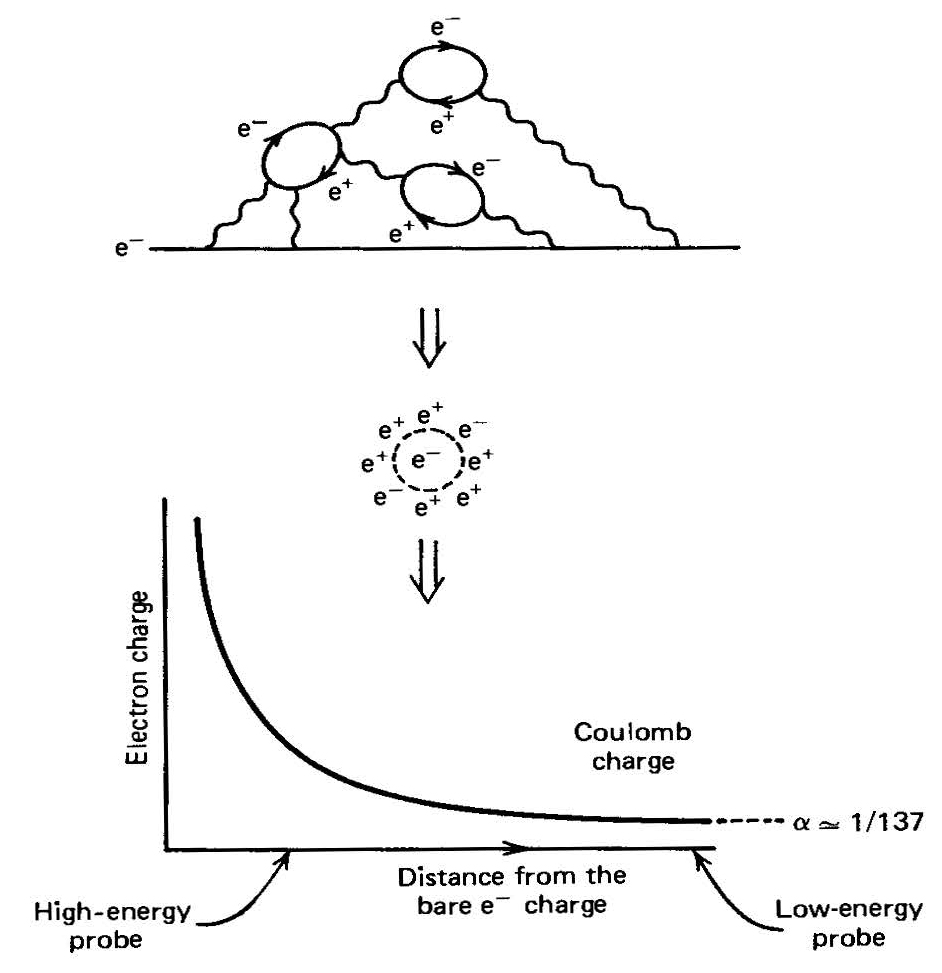
\includegraphics[width=10cm]{img/Running-coupling-constant-QED.jpg}
\end{figure}

Suppose that we want to determine the charge of the electron by measuring the Coulomb force experienced by a test charge. The result will depend on where we place the test charge: when moving the test charge closer to the electron, we penetrate the cloud of positrons that screens the electron's charge. Therefore, the closer one approaches the electron, the larger is the charge one measures. In QFT the vacuum surrounding the electron has become a polarizable medium. The situation is analogous to that of a negative charge in a dielectric medium: the electron-positron pairs respond to the presence of the electron like the polarized molecules do in the dielectric. This effect is known as charge screening; as a result the ``measured charge'' depends on the distance one is probing the electron. 

In the QED we discussed electron-proton scattering and we derived that this can be described using a Coulomb potential in the form
\[V(r)=\frac{\alpha}r\]
where $\alpha_0$ is the usual E-M coupling constant. We seen that when we renormalize QED (compare for instance with eq.~\eqref{eqn:correction-charge-NLO-QED}) the charge is modified by vacuum polarization loop in the photon propagator. Indeed, more in general, for higher order we can describe the interaction in the renormalized theory through a modified coulomb potential, where $\alpha$ is substituted by
\[\alpha_{EM}(s)=\frac{\alpha}{1-\frac{\alpha}{3\pi}\log({s}/{\mu_0^2})}\]
where $\mu_0$ is some term given by renormalization called renormalization or reference momentum, and $s$ is the Mandelstam variable associated to the momentum of the propagator.

The term $\alpha_{EM}(s)$ is called \textbf{running coupling constant} since it depends on the energy of the photon, and describes how the effective charge depends on the separation of the two charged. Then, by summing part of all orders of perturbation theory, we have obtained the charge screening of electrodynamics. As $s$ increases, the photon sees more and more charge until, at some astronomically large but finite $s$, the coupling $\alpha_{EM}(s)$ is infinite. such point is called \textbf{Landau pole} and corresponds usually to $\sqrt s=10^{286}$eV. However, by inserting numerical values, we find that for all practically attaindable $s$, the variation of $\alpha_{EM}$ with $s$ is extremely small; $\alpha_{EM}$ increases from $1/137$ very slowly as $s$ increases. Of course, as $s$ increases, other loops (formed, for example, by a $\mu^+\mu^-$-pair or a $\bar u u$-quark pair) will also contribute to the variation. The energy 

\subsubsection{Confinement and asymptotic freedom in QCD}

One can carry through the same calculation for the color charge of a quark. Color screening would be a carbon copy of charge screening if it were not for the new configurations involving gluons turning into pairs of gluons, as shown in next figure:

\begin{figure}[H]
\centering
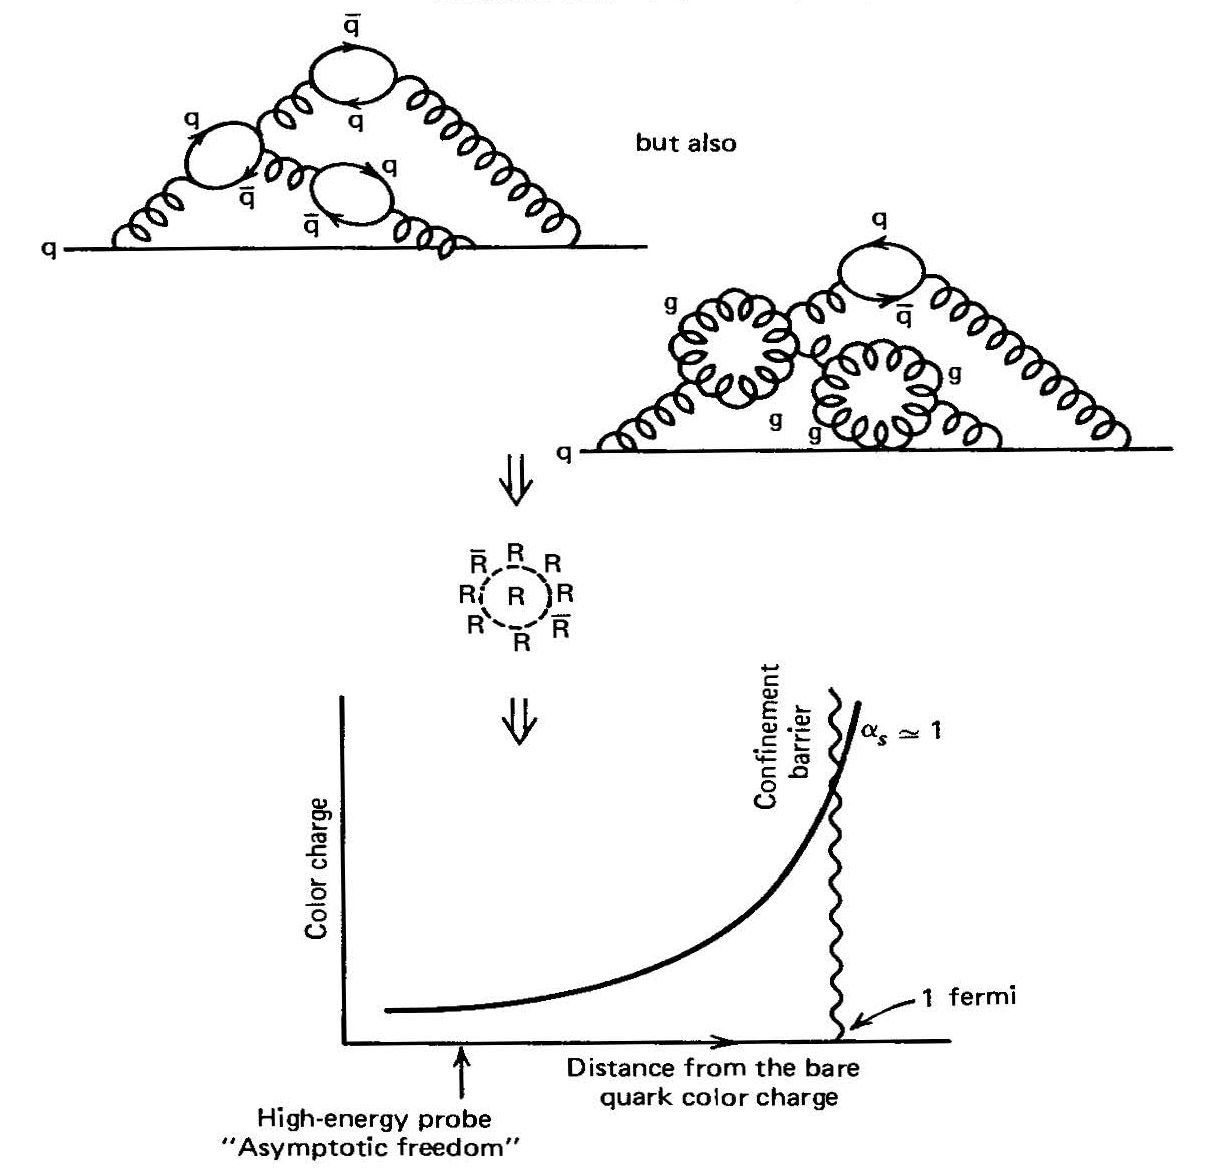
\includegraphics[width=11cm]{img/Running-coupling-constant-QCD.jpg}
\end{figure}

The gluons, themselves carriers of color, also spread out the effective color charge of the quark. It turns out that the additional diagrams reverse the familiar result of quantum electrodynamics: a red charge is preferentially surrounded by other red charges. We now repeat the measure made with the probe for color changes. By moving out test probe closer to the original red quark, the probe penetrates a sphere of predominantly red charge and the amount of red charge measured decreases. The resulting ``antiscreening'' effect is referred to as \textbf{asymptotic freedom}. Asymptotically, two red quarks interact (i.e. for very small separations) through color fields of reduced strength and approach a state where they behave as essentially free, noninteracting particles. 

Doing explicit calculation in QCD, after we renormalized the theory, the running coupling term for strong interactions shows following dependence on $s$ (the label $s$ in $\alpha_s$ indicate that this is the coupling for the \emph{s}trong interaction):
\[\alpha_s(s)=\frac{\alpha_s}{1+\frac{\alpha_s}{12\pi}(33-2n_f)\log(s/\mu_0^2)}\]
where $n_f$ is the number of quark flavours at energy $s$ (in our world $n_f\leq6$). Only in a world with more that 16 quarks flavours is the sign of the coefficient the same as in QED. Then $\alpha_s$ decreases with increasing $s$ and therefore becomes small for short-distance interactions. We say that the theory is ``\textbf{asymptotically free}''.
One parameter, $\mu_0$, with the dimension of mass, remains as a relic of the renormalization. We see that at sufficiently low $s$, the effective coupling will become large. This implies that in such case the perturbative approach doesn't work. It is costumary to denote the $s$ scale at which this happens by $\Lambda_{QCD}^2$. Typical scale of this value is $\Lambda_{QCD}\simeq200MeV$ and corresponds to a distance of $\lambda \simeq1$fm.

For $s$ values much larger than  $\Lambda_{QCD}^2$, the effective coupling is small and perturbative description in terms of quarks and gluons interacting weakly makes sense. For $s$ of order $\Lambda_{QCD}^2$, we cannot make such a picture, since quarks and gluons will arrange themselves into strongly bound cluster, namely, hadrons. Thus, we can think of $\Lambda_{QCD}$ as marking the boundary between a world of quasi-free quarks and gluons, and the world of pions, protons, and so on. 

\subsection{$e^+e^-\,\rightarrow\,$ hadrons production}
\textsf{Peskin 5.1; Halzen, sec. 11.1}\\

The simples reaction involving quarks is the production of quarks pairs in $e^+e^-$ annihilation, which at most elementary level is a straightforward generalization of the process $e^+e^-\,\rightarrow\,f^+f^-$. Indeed, according to QCD, the simplest $e^+e^-$ process that ends in hadrons is 
\[e^+e^-\,\rightarrow\,q\bar q\]
the annihilation of an electron and a positron, through a virtual photon, into a quark-antiquark pair. After they are created, the quarks interact with one another through their strong forces, producing more quark pairs. Eventually the quark and antiquarks combine to form some number of mesons and baryons. 

To adapt the result we obtained for $e^+e^-\,\rightarrow\,f^+f^-$ scattering in sec.~\ref{sec:electr-to-muon-scatt-QED} to handle the case of quarks, we must make three modifications:
\begin{enumerate}
\item replace the $f$ charge with the quark charge;
\item count each quark three times, one for each color;
\item include the effects of the strong interactions of the produced quark and antiquark
\end{enumerate}
Counting colors is necessary because experiments measure only the total cross section for production of all three colors (since hadrons are detected colorless). Surely the third modification is extremely difficult to make, but in high-energy limit, the effect of the strong interaction on the quark production process can be completely neglected, thanks to asymptotic freedom of the theory. The only effect of the strong interaction in this limit is to dress up the final-state quarks into bunches of hadrons. 

Starting from the total scattering amplitude in the UR regime for the $e^+e^-\,\rightarrow\,f^+f^-$ given by eq.~\eqref{eqn:electr-muon-scatt-QED-UR} (we consider only first order terms):
\[ \sigma_{e^+e^-\,\rightarrow\,f^+f^-} = \frac{4 \pi \alpha_{EM}^2}{3s}
\]
it is conventional to define, in the asymptotic limit
\[R=\frac{\sigma_{e^+e^-\,\rightarrow\,\text{hadrons}}}{\sigma_{e^+e^-\,\rightarrow\,f^+f^-}}=N_c\sum_q(q_q^2)\]
where $N_c$ is the number of colors for quarks (in our theory $N_c=3$) and the sum runs over all quarks whose masses are smaller that $E_{cm}/2$ and $q_q$ is the fractional charge of these quarks (respect to the electron one). 
For instance
\begin{alignat*}{3}
R&=3\p{\p{\frac23}^2+\p{\frac13}^2+\p{\frac13}^2}=2	\qquad&&\text{for }u,\,d,\,s\\
&=2+3\p{\frac23}^2=\frac{10}3	&&\text{for }u,\,d,\,s,\,c\\
&=\frac{10}3+3\p{\frac13}^2=\frac{11}3	&&\text{for }u,\,d,\,s,\,c,\,b
\end{alignat*}
In fig.~\ref{fig:elect-quark-scatt} these prediction are compared to the measurements of $R$.  The value $R\simeq 2$ is apparent below the threshold for producing charmed particles at $\sqrt s=2(m_c+m_u)\simeq3.7$GeV. Above the threshold for all five quark flavors ($\sqrt s>m_b\simeq10$GeV),$R\simeq\frac{11}3$ as predicted. These measurements confirm that there are three color of quarks, since $R=\frac{11}3$ would be reduced by a factor 3 if there was only one color. 

When $E_{cm}/2$ is in the vicinity of one of quark masses, the strong interaction cause large deviation from this formula. The most dramatic such effect is the appearance of bound states just below $E_{cm}=2m_q$, manifested as very sharp spikes in the cross section.

These results for $R$ will be modified when we take into account correction due to the running coupling. In particular, the result we obtained holds only at leading order. 

\begin{figure}[H]
\centering
\includegraphics[width=15.5cm]{img/electr-quark-scatt.jpg}
\caption{Ratio $R$ as a function of the total $e^-e^+$ center-of-mass energy. (The sharp peaks correspond to the production of narrow resonance just below or near the flavor thresholds)}
\label{fig:elect-quark-scatt}
\end{figure}

\subsection{Quark-quark scattering hard process and QCD potential}

\textsf{Schwartz, sec. 26.2; Peskin, sec. 17.4}\\

To get a feeling for how QCD differs from QED, we examine the tree-level potential between quarks. In QED, we saw in sec.\ref{sec:scatt-Rutherf} that the potential could be extracted from Coulomb scattering $e^-p^+\rightarrow e^-p^+$, which has a contributions from $t$-channel photons. Let us now consider the process $u\bar d\,\rightarrow\,u\bar d$ where $u$ and $d$ are up and down quarks. These are Dirac spinors transforming in the fundamental representation of QCD. The sign and the strength of the potential extracted from the $t$ channel exchange will tell us whether the transition is attractive or repulsive, and thus whether bound states can exist. 

The tree-level diagram for elastic $u\bar d\,\rightarrow\,u\bar d$ scattering in QCD is

\begin{equation*}
\begin{tikzpicture}[baseline=(i)]
  \begin{feynman}[large]
    \vertex (f1) {$u$, {\footnotesize $i$}};
    \vertex [label={[label distance=0.2cm]90:{\footnotesize$\mu,\,a$}}] at ([shift={(315:2.5)}]f1)  (u);
    \vertex [label={[label distance=0.1cm]270:{\footnotesize$\nu,\,b$}}] at ([shift={(270:2)}]u) (d);
    \vertex [below right=of d] (f2) {$\bar d$, {\footnotesize $l$}};
    \vertex [below left=of d] (b1){$\bar d$, {\footnotesize $k$}};
    \vertex [above right=of u] (b2){$u$, {\footnotesize $j$}};
    \vertex at ([shift={(270:1)}]u)(i);
    
    \diagram*{
      (f1) -- [fermion, momentum'={[arrow shorten=0.25]\(p\)}] (u) -- [gluon, momentum={[arrow shorten=0.3]\(\sqrt{t}=(p-p')=(q'-q)\)}] (d) -- [fermion, momentum={[arrow shorten=0.2]\(q'\)}](f2),
      (u) -- [fermion, momentum'={[arrow shorten=0.3]\(p'\)}] (b2),
      (b1) -- [fermion, momentum={[arrow shorten=0.2]\(q\)}] (d),
      };
  \end{feynman}
\end{tikzpicture}
\end{equation*}
where labels $a,b$ and $i,j,k,l$ indicate colors respectively of quarks and gluons

Notice that a similar diagram, with a photon instead of the gluon, is given by QED, but comparing  coupling constant for typical values of energies we see that QED contributions can be neglected
\[\alpha_s(s)\simeq 0.12\quad\gg\quad\alpha_{EM}(s)\simeq 0.007\]

The Ferynman amplitude for this QCD process is given by
\[\mathcal M=(ig_s)^2\p{\bar u_j(p')\gamma^\mu u_i(p)}\p{v_k(q)\gamma^\nu v_l(q')}\sum_{ab}\p{T^a}_{ji}\p{T^b}_{kl}D_{\mu\nu}^{ab}(t)\]

And using eq.~\eqref{eqn:gluon-propagator} with $\xi=1$ we obtain

\[\mathcal M=\frac{ig_s^2}{t}\sum_a\p{T^a}_{ji}\p{T^a}_{kl}\p{\bar u_j(p')\gamma^\mu u_i(p)}\p{v_k(q)\gamma^\nu v_l(q')}\]

Notice that $\frac1t$ behaviour of the amplitude is the same as for process $e^+e^-\rightarrow e^+e^-$ in QED, therefore also the interaction given by gluon is Coulomb like. 

To understand the $\p{T^a}_{ji}\p{T^b}_{kl}$ coefficient, let us consider different choices for the color of the incoming $u$ and $\bar d$ quarks. For example, suppose the incoming $u$ is red and the incoming $\bar d$ is anti-green ($i=1$, $k=2$). Then, by explicit computation using Gell-Mann matrices we obtain
\[\sum_a\p{T^a}_{j1}\p{T^a}_{2l}=\left(\begin{array}{ccc}0 & 1/6 & 0 \\0 & 0 & 0 \\0 & 0 & 0\end{array}\right)_{jl}=-\frac16\delta_{j1}\delta_{2l}\]
so that $j=1$ and $l=2$. That is, the final state must also have a red quark and a green anti-quark. Of course, just because color is conserved. Since $\sum_a\p{T^a}_{11}\p{T^a}_{22}=-\frac16$, the $t$-channel diagram has the opposite sign from the $e^-p^+$ case and the potential is therefore repulsive (as it would be for say $e^+p^+$ scattering). Indeed it is impossible to have stable colored states since in this case potential is repulsive.

On the other hand, suppose both $u$ is red and $\bar d$ is anti-red. Then the initial state is a color singlet (color and anti-color cancel each other). In this case $i=1$ and $k=1$ and 
\begin{equation}\label{eqn:colorless-matrix-contr}
\sum_a\p{T^a}_{j1}\p{T^a}_{2l}=\left(\begin{array}{ccc}1/3 & 0 & 0 \\0 & 1/2 & 0 \\0 & 0 & 1/2\end{array}\right)_{jl}
\end{equation}
so the final state can be red/anti-red, blue/anti-blue or green/anti-green. In any of these cases, the color factor will have a positive coefficient and the potential will be attractive. 

To get the overall strength of the potential, let's consider the most general color singlet state:
\[\ket1=\frac{1}{\sqrt3}\big(\ket{r\bar r}+\ket{b\bar b}+\ket{g\bar g}\big)\]
Summing over all the possibilities for $\ket{r\bar r}\,\rightarrow\,$ anything gives a factor 4/3 from the trace of eq.~\eqref{eqn:colorless-matrix-contr}. We then get three times this (for the three collors) multiplied by the normalization $\p{\frac1{\sqrt3}}^2$. Therefore the potentia is
\[V_s(r)=-\frac{N_c}{(\sqrt 3)^2}\underbrace{\Tr[\sum_aT^aT^a]}_{4/3}\frac{\alpha_s}r=-\frac43\frac{\alpha_s}r\]
Then only the color singlet channel is attractive is consistent with the observational fact we do not find colored mesons in nature. 

Let's compute the total scattering amplitude in the high energy limit. The unpolarized Feyman amplitude must average also over all possible color of initial states:
\begin{align*}
\vert\overline{\mathcal M} \vert^2
&=\p{\frac13}^2\sum_{\text{color}}\p{\frac12}^2\sum_{\text{spin}}\p{\frac{g_s^2}t}^2\vert(\text{$u$-current})(\text{$\bar d$-current})\vert^2\vert\sum_a\p{T^a}_{ji}\p{T^a}_{kl}\vert^2\\
&=\frac14\p{\frac{g_s^2}t}^2\Tr[\text{$u$-current}]\Tr[\text{$\bar d$-current}]\frac19\sum_{ab}\sum_{ij}\p{T^a}_{ji}\p{T^b}_{ij}\sum_{kl}\p{T^a}_{kl}\p{T^b}_{lk}
\end{align*}
where we used $\p{T^a}_{ij}^*=\p{T^a}_{ji}$. 
We can simplify calculation using the result we already know from QED process $e^-\mu^+\rightarrow e^-\mu^+$
\begin{align*}
\vert\overline{\mathcal M} \vert^2
&=\frac19\sum_{ab}\Tr[T^aT^b]\Tr[T^aT^b]\p{\frac{\alpha_s}{\alpha_{EM}}}^2\vert\overline{\mathcal M} \vert^2_{e^-\mu^+}\\
&=\frac19\sum_{ab}\p{\frac12\delta_{ab}}\p{\frac12\delta_{ab}}\p{\frac{\alpha_s}{\alpha_{EM}}}^2\vert\overline{\mathcal M} \vert^2_{e^-\mu^+}\\
&=\frac19\frac84\p{\frac{\alpha_s}{\alpha_{EM}}}^2\vert\overline{\mathcal M} \vert^2_{e^-\mu^+}
=\frac29\p{\frac{\alpha_s}{\alpha_{EM}}}^2\vert\overline{\mathcal M} \vert^2_{e^-\mu^+}
\end{align*}
Finally (recall that we are working in the high energy limit, i.e. $m_f=0$):
\[\vert\overline{\mathcal M} \vert^2_{u\bar d}=\frac{64\pi^2}9\alpha_s^2\p{\frac{s^2+u^2}{t^2}}\]
and
\[{\p{\frac{\de\overline\sigma}{\de\Omega}}}_{u\bar d}=\frac{\alpha_s^2}{9t}\p{\frac{s^2+u^2}{t^2}}\]















\end{document}